\chapter{Hệ thống đề xuất}
\label{chap:hethong}

Chương này mô tả Farmery từ góc nhìn nghiệp vụ và yêu cầu: ngữ cảnh nghiệp vụ, quy trình và chính sách (mục~\ref{sec:ngucanh}); tổng quan hệ thống, vấn đề nghiên cứu và thách thức (mục~\ref{sec:motahethong}); bộ yêu cầu chức năng, phi chức năng và dữ liệu (mục~\ref{sec:yeucau}). Mô hình hóa và thiết kế chi tiết ở Chương~\ref{chap:phantich}.

\section{Ngữ cảnh nghiệp vụ}
\label{sec:ngucanh}

\subsection{Mô hình kinh doanh}
\label{sec:businessmodelcanvas}

Farmery vận hành hai luồng thương mại trên cùng một tập nguồn cung là nông dân và hợp tác xã đã xác thực. Hai luồng khác nhau ở điểm căn bản: \textbf{ai sở hữu hàng trong lúc giao dịch}, kéo theo khác biệt về định giá, doanh thu và bên chịu rủi ro (Bảng~\ref{tab:hailuong}).

\begingroup
\tblsetup\tblzebra
\begin{table}[H]
\centering
\small
\caption{Đối chiếu hai luồng thương mại của Farmery}
\label{tab:hailuong}
\begin{tabular}{L{3.75cm} L{5.58cm} L{5.57cm}}
\toprule
\rowcolor{tblheadbg}
\textbf{Tiêu chí} & \textbf{Bán sỉ --- sàn (3P)} & \textbf{Bán lẻ --- thu mua bán lại (1P)} \\
\midrule
Quyền sở hữu hàng & Nhà cung cấp giữ tới khi giao & Farmery thu mua theo lô \\
Bên định giá & Nhà cung cấp & Farmery \\
Doanh thu nền tảng & Hoa hồng theo đơn & Chênh lệch giá mua--bán \\
Rủi ro tồn kho, hao hụt & Nhà cung cấp chịu & Farmery chịu \\
Trách nhiệm chất lượng trước người mua & Nhà cung cấp & Farmery \\
Nhu cầu vốn lưu động & Không & Có --- đánh đổi lớn nhất \\
Bên mua & Doanh nghiệp mua sỉ & Người tiêu dùng cá nhân \\
\bottomrule
\end{tabular}
\end{table}
\endgroup

\noindent\textbf{Vì sao ghép được hai luồng.} Với đơn sỉ khối lượng lớn, nhà cung cấp giao thẳng cho doanh nghiệp là hiệu quả nhất, nền tảng chỉ đứng giữa bảo đảm minh bạch. Với đơn lẻ vài ki-lô-gam, phần lớn nông dân và hợp tác xã không đủ năng lực phân loại, đóng gói, xử lý từng đơn nhỏ; luồng 1P gánh phần việc đó, đổi lại phải bỏ vốn và chịu rủi ro tồn kho. Hai luồng hỗ trợ nhau một chiều: lô đăng bán sỉ sắp hết hạn bảo quản mà chưa có người mua có thể được nhân viên thu mua mua lại với giá chiết khấu. Chiều ngược lại không mở: Farmery không bán sỉ, kể cả hàng bán lẻ tồn dư (xả bằng giảm giá ở kênh bán lẻ), để nền tảng không dùng vị thế vận hành sàn cạnh tranh với chính nhà cung cấp. Phần hiện thực tập trung vào trục bán lẻ đầu--cuối (mục~\ref{sec:phamvi}).

Bảng~\ref{tab:bmc} trình bày mô hình theo khung Business Model Canvas (mục~\ref{subsec:businessmodel}); ký hiệu 3P, 1P chỉ luồng tương ứng, mục không ghi ký hiệu dùng chung cho cả hai.

\begingroup
\tblsetup
\begin{longtable}{L{2.80cm} L{12.45cm}}
\caption{Business Model Canvas của Farmery}
\label{tab:bmc} \\
\toprule
\rowcolor{tblheadbg}
\textbf{Khối} & \textbf{Nội dung} \\
\midrule
\endfirsthead
\toprule
\rowcolor{tblheadbg}
\textbf{Khối} & \textbf{Nội dung} \\
\midrule
\endhead
\bottomrule
\endfoot
Phân khúc khách hàng & Nhà cung cấp là nông dân, hợp tác xã tại vùng trồng thí điểm; khách sỉ là nhà hàng, siêu thị, nhà phân phối (3P); khách lẻ là người tiêu dùng cá nhân tại TP.HCM (1P). \\
Giá trị đề xuất & \emph{Nhà cung cấp:} hai lựa chọn đầu ra thay vì phụ thuộc thương lái. \emph{Khách sỉ:} nguồn cung đã xác thực chứng nhận, giá bậc minh bạch, truy xuất tới từng lô. \emph{Khách lẻ:} hàng đóng gói kèm tem truy xuất, một đầu mối chịu trách nhiệm chất lượng và đổi trả. \\
Quan hệ khách hàng & Tự phục vụ trên ứng dụng, khiếu nại gắn với từng đơn; hỗ trợ chung qua Zalo OA; nhân sự đồng hành khách sỉ; hỗ trợ vùng cho nhà cung cấp ít rành công nghệ. \\
Kênh phân phối & Ứng dụng mua hàng (PWA); mạng xã hội, tối ưu tìm kiếm; hội nông dân, hợp tác xã, OCOP; tiếp cận trực tiếp khách sỉ; đội thu mua tại vùng trồng (1P). \\
Hoạt động chính & Kiểm duyệt nhà cung cấp, sản phẩm, chứng nhận; kết nối cung cầu, báo giá và hợp đồng sỉ (3P); thu mua theo lô, nghiệm thu, đóng gói kèm QR, định giá, quản lý tồn kho, điều phối xe lạnh, đổi trả (1P); vận hành nền tảng, uy tín và mô-đun AI. \\
Nguồn lực chính & Ứng dụng mua hàng, ứng dụng nội bộ, hạ tầng AI; dữ liệu truy xuất và nhật ký canh tác tích lũy; đội kiểm duyệt, vận hành, hỗ trợ vùng; vốn lưu động thu mua (1P); kho sơ chế nhỏ tại vùng trồng. \\
Đối tác chính & Đơn vị xe lạnh theo chuyến và vận chuyển nội thành (3PL); cổng thanh toán, hóa đơn điện tử; hệ thống truy xuất của Bộ Nông nghiệp và Môi trường (khi được cấp quyền); cơ quan cấp VietGAP, GlobalGAP; hội nông dân, hợp tác xã; OCOP. \\
Dòng doanh thu & Hoa hồng đơn sỉ thành công (3P); chênh lệch giá mua--bán lẻ (1P); cước giao lẻ chỉ bù chi phí, miễn khi vượt ngưỡng. Không thu phí đăng ký, duy trì tài khoản hay xử lý đơn với nhà cung cấp. Mức phí theo \emph{Biểu phí công bố} (FR10.6). \\
Cơ cấu chi phí & Giá vốn hàng mua vào (lớn nhất), hao hụt và hàng không bán hết, đóng gói, xe lạnh và cước 3PL (1P); hạ tầng và đội kỹ thuật; nhân sự kiểm duyệt, chăm sóc khách hàng, thu mua; marketing; tích hợp bên thứ ba. \\
\end{longtable}
\endgroup

Gói hiển thị nổi bật gắn nhãn ``Tài trợ'' và dịch vụ kho mở cho nhà cung cấp để ở hướng phát triển (Chương~\ref{chap:ketluan}); Farmery không bán dịch vụ ``xác thực chứng nhận nhanh'' vì sẽ làm nhãn chứng nhận mất tính độc lập, trái với lập luận niềm tin của V4 (mục~\ref{sec:vande}).

\noindent\textbf{Điều kiện hòa vốn của luồng 1P.} Gọi $g$ là giá thu mua một ki-lô-gam, $h$ là tỷ lệ hao hụt từ nghiệm thu tới lúc bán ($0 \le h < 1$), $c_{\text{đg}}$ là chi phí đóng gói một ki-lô-gam, $c_{\text{vh}}$ là chi phí vận hành một đơn và $q$ là số ki-lô-gam trung bình mỗi đơn. Giá bán lẻ $p$ chỉ có lãi khi:
\[
p - g \;\ge\; \underbrace{\frac{h}{1-h}\,g}_{\text{hao hụt}} \;+\; \underbrace{c_{\text{đg}}}_{\text{đóng gói}} \;+\; \underbrace{\frac{c_{\text{vh}}}{q}}_{\text{vận hành mỗi đơn}}
\]
Cước giao không có trong vế phải vì đã thu đủ từ khách. Với tổn thất sau thu hoạch 20--40\% (V3), riêng số hạng hao hụt đã bằng 25--67\% giá thu mua; thiết kế luồng 1P vì vậy xoay quanh việc giữ $h$ thấp: chỉ thu mua lượng bán được trong thời hạn bảo quản, xuất theo FEFO, và rút ngắn thời gian hàng nằm trên đường bằng chuyến trung chuyển cố định.

\subsection{Quy trình nghiệp vụ và quy tắc nghiệp vụ}
\label{sec:quytrinhnghiepvu}

Mười quy trình dưới đây ghi tác nhân, điều kiện chuyển bước và ngoại lệ chính; hai quy trình thu mua và đặt hàng có sơ đồ hoạt động ở mục~\ref{subsec:mohinhquytrinh}. Phần \emph{(chỉ thiết kế)} được tổng hợp ở Bảng~\ref{tab:chi-thiet-ke}.

\noindent\textbf{1. Đăng ký và xác thực nhà cung cấp, kiểm duyệt chứng nhận.}
\begin{itemize}
    \item \emph{Luồng chính:} nhà cung cấp đăng ký, nhập định danh (CCCD, hoặc mã số thuế với hợp tác xã), thông tin trang trại và loại người bán cho nghĩa vụ thuế (FR2.4); xác thực OTP qua email; làm eKYC bằng ảnh giấy tờ và chân dung (FR1.4); tải chứng nhận VietGAP, GlobalGAP, hữu cơ, OCOP, HACCP kèm mã số, cơ quan cấp, ngày hết hạn.
    \item \emph{Kiểm duyệt ba tầng:} hệ thống kiểm định dạng mã vùng trồng; kiểm duyệt viên đối chiếu mã với cổng công bố của Bộ Nông nghiệp và Môi trường; giấy chứng nhận được duyệt hồ sơ thủ công. eKYC đạt thì tài khoản ``Đã xác thực'' và được đăng bán; không đạt thì nhận lý do và hướng dẫn bổ sung.
    \item \emph{Quy tắc, ngoại lệ:} nhập sai OTP quá 5 lần thì khóa 30 phút; chứng nhận hết hạn thì nhãn trên sản phẩm bị ẩn (sản phẩm không bị gỡ); chứng nhận giả thì khóa vĩnh viễn, không đăng ký lại bằng cùng định danh.
\end{itemize}

\noindent\textbf{2. Đăng và kiểm duyệt sản phẩm, sinh mã QR.}
\begin{itemize}
    \item \emph{Luồng chính:} nhà cung cấp đã xác thực tạo sản phẩm (tên, mô tả, ảnh, đơn vị tính, giá lẻ, giá sỉ theo bậc, sản lượng, ngày thu hoạch dự kiến) và ghi nhật ký canh tác theo giai đoạn, gắn với một lô. Hệ thống kiểm tra sơ bộ (ảnh trùng, từ khóa cấm, giá bất thường); kiểm duyệt viên duyệt thủ công sản phẩm mới hoặc nhà cung cấp chưa có lịch sử (nhà cung cấp có uy tín được hậu kiểm).
    \item \emph{Kết quả:} hệ thống sinh mã QR duy nhất cho từng lô, dẫn tới trang truy xuất công khai (hồ sơ, chứng nhận, nhật ký, mốc vận chuyển); lô được mở bán ngay sau duyệt nội bộ.
    \item \emph{Quy tắc:} chỉ hiển thị công khai khi có tối thiểu một bản ghi nhật ký gần nhất và ảnh thực tế; thay đổi trọng yếu sau duyệt (giá đổi quá 20\% hoặc mô tả chất lượng đổi) phải duyệt lại.
\end{itemize}
Hàng đăng bán phải đúng là nông sản, bảo đảm bằng bốn lớp: (L1) \emph{danh mục đóng} --- sản phẩm gắn danh mục lá do quản trị viên định nghĩa theo mục~\ref{subsec:dinhnghianongsan}, mỗi danh mục quy định đơn vị tính và trường bắt buộc; (L2) \emph{danh sách loại trừ} công khai ngay tại biểu mẫu đăng bán; (L3) \emph{kiểm duyệt trước khi hiển thị}, nhóm chế biến sâu bắt buộc có bản tự công bố; (L4) \emph{hậu kiểm bằng báo cáo của người mua} \emph{(chỉ thiết kế)}. Chế tài tăng dần: ẩn sản phẩm và yêu cầu phân loại lại; tái phạm thì cảnh cáo, trừ điểm uy tín; cố tình đăng hàng bị loại trừ thì khóa quyền đăng bán.

\noindent\textbf{3. Thu mua vào kho.}
\begin{itemize}
    \item \emph{Đặt mua:} nhà cung cấp công bố lô sắp thu hoạch kèm sản lượng và giá chào. Nhân viên thu mua đối chiếu chào giá cùng loại và tồn kho (có dự báo giá \emph{chỉ thiết kế}), lập đơn thu mua; đơn chỉ có hiệu lực khi \textbf{nhà cung cấp xác nhận}, từ đó sản lượng trong đơn được giữ chỗ, không chào sỉ được nữa.
    \item \emph{Nhập kho:} nhà cung cấp tự đưa hàng về kho sơ chế (xe gom \emph{chỉ thiết kế}); nhân viên kho nghiệm thu, phần đạt thành một \emph{dòng tồn} của Farmery giữ nguyên mã lô, nhật ký, QR; nhà cung cấp được thanh toán theo sản lượng đã nghiệm thu, không chờ hàng bán được.
    \item \emph{Đóng gói, đặt giá:} nhân viên kho đóng gói thành đơn vị bán lẻ trong một bước, dán tem gồm QR và nhãn bắt buộc (tên hàng, đơn vị chịu trách nhiệm, xuất xứ, định lượng, ngày đóng gói, hạn dùng, bảo quản), ghi hao hụt vào sổ nhập xuất; nhân viên thu mua đặt giá theo điều kiện hòa vốn rồi mở bán.
    \item \emph{Ngoại lệ:} nhà cung cấp không xác nhận đúng hạn thì đơn tự hủy; chất lượng không đạt thì từ chối hoặc nhận giá điều chỉnh, lệch nghiêm trọng ghi vào lịch sử uy tín; lô tồn lâu hoặc cận hạn thì cảnh báo để giảm giá xả.
\end{itemize}

\noindent\textbf{4. Bán lẻ.}
\begin{itemize}
    \item \emph{Tìm và đặt:} khách lẻ tìm bằng câu tự nhiên hoặc từ khóa (không dấu, gõ sai vẫn tìm được), lọc theo danh mục, vùng, chứng nhận, giá; xem chi tiết kèm tóm tắt truy xuất; thêm vào giỏ trong giới hạn tồn trên dòng tồn của Farmery. Ở bước thanh toán, hệ thống hiển thị đủ tiền hàng, thuế, cước trước khi xác nhận; COD chỉ cho đơn dưới ngưỡng và tài khoản chưa từng từ chối nhận hàng.
    \item \emph{Giữ chỗ và giao:} hệ thống giữ chỗ và trừ tồn trong một giao dịch có khóa để tránh bán vượt. Đơn trước \emph{giờ chốt} hằng ngày được đóng gói, dán tem và lên \emph{chuyến trung chuyển} về TP.HCM trong ngày, đơn sau giờ chốt vào chuyến kế tiếp; 3PL nội thành giao theo khung giờ khách chọn.
    \item \emph{Theo dõi và hoàn tất:} dòng thời gian tám trạng thái (Đã đặt $\rightarrow$ Đã thanh toán $\rightarrow$ Đang đóng gói $\rightarrow$ Lên chuyến trung chuyển $\rightarrow$ 3PL đã nhận $\rightarrow$ Đang giao $\rightarrow$ Đã giao $\rightarrow$ Hoàn tất hoặc Khiếu nại). Hết thời hạn khiếu nại mà không có khiếu nại, đơn Hoàn tất, phát hành hóa đơn điện tử (giả lập) và mở quyền đánh giá.
    \item \emph{Ngoại lệ:} thanh toán thất bại giữ đơn tối đa 15 phút rồi tự hủy và nhả tồn; hủy trước đóng gói thì nhả tồn, hoàn tiền; từ chối COD không có lý do chất lượng thì mất quyền COD; nhiều đơn vượt tồn thì ưu tiên đơn xác nhận trước, các đơn còn lại hủy kèm thông báo.
\end{itemize}

\noindent\textbf{5. Đánh giá sản phẩm và nhà cung cấp.}\label{subsec:danhgianghiepvu}
\begin{itemize}
    \item \emph{Luồng chính:} chỉ người mua đã nhận hàng được đánh giá (điểm 1--5 sao, bình luận, ảnh). Hệ thống kiểm tra sơ bộ và dùng luật ngưỡng gắn cờ đánh giá nghi vấn cho kiểm duyệt viên duyệt trước khi công khai hoặc ẩn.
    \item \emph{Điểm uy tín:} chuẩn hóa về thang 0--100, là trung bình có trọng số của các đánh giá hợp lệ trong 6 tháng gần nhất, đánh giá gần đây và đơn giá trị lớn có trọng số cao hơn. Thang 0--100 phân biệt tốt hơn thang sao vốn dồn cụm ở 4--5 sao \parencite{springer_article}; trọng số thời gian để điểm phản ánh chất lượng gần đây.
    \item \emph{Quy tắc:} nhà cung cấp từ 80/100 trở lên được hậu kiểm nhanh khi đăng sản phẩm mới và ưu tiên hiển thị (ngưỡng đặt cao vì hậu kiểm nhanh giảm kiểm soát trước đăng bán); thao tác thao túng đánh giá bị xử lý theo quy trình 10.
\end{itemize}

\noindent\textbf{6. Bán sỉ (B2B).}
\begin{itemize}
    \item \emph{Báo giá:} nhà cung cấp công bố bảng giá bậc, MOQ và lịch giao. Doanh nghiệp mua sỉ gửi yêu cầu báo giá (RFQ); nếu chưa đạt MOQ, hệ thống gợi ý gộp đơn hoặc chuyển sang bán lẻ. Nhà cung cấp phản hồi một báo giá (FR6.2); bên mua chấp nhận hoặc từ chối.
    \item \emph{Hợp đồng và giao hàng:} khi chấp nhận, hệ thống sinh hợp đồng một lần từ mẫu chuẩn kèm phạt vi phạm, điều khoản thanh toán và mã băm; hai bên \emph{xác nhận giao kết} bằng mã dùng một lần qua email, hệ thống lưu tài khoản, thời điểm và mã băm văn bản. Nhà cung cấp tự giao hoặc thuê 3PL \textbf{một đợt}, xuất hóa đơn; bên mua xác nhận nhận hàng và thanh toán qua cổng; Farmery ghi hoa hồng và xuất hóa đơn dịch vụ.
    \item \emph{Chỉ thiết kế:} thương lượng nhiều vòng, nhiều phiên bản hợp đồng, giao nhiều đợt, ký quỹ, khấu trừ thuế thay (FR6.2, FR6.3, FR6.5, FR7.3, FR7.4).
    \item \emph{Ngoại lệ:} giao thiếu hoặc trễ thì phạt theo hợp đồng và ghi vào uy tín; bên mua chậm thanh toán thì nhắc và có thể tạm khóa RFQ mới; từ chối một phần thì hàng về đúng dòng tồn nguồn, tranh chấp xử lý theo hợp đồng (FR10.3).
\end{itemize}

\noindent\textbf{7. Quản lý tồn kho theo dòng tồn.}
\begin{itemize}
    \item \emph{Lô và dòng tồn:} một lô là đơn vị truy xuất (một mã lô, nhật ký, QR), nhưng hàng cùng lô có thể ở nhiều nơi và thuộc nhiều chủ, nên tồn kho ghi trên \emph{dòng tồn} xác định lô, chủ sở hữu và nơi chứa. Ví dụ lô 1.000 kg của một hợp tác xã, khi Farmery thu mua 300 kg thì có hai dòng: 700 kg của hợp tác xã (chỉ bán sỉ) và 300 kg của Farmery tại kho sơ chế (chỉ bán lẻ).
    \item \emph{Sổ nhập xuất:} mọi thay đổi số lượng đi qua sổ ghi nguồn giao dịch (nhập thu mua, bán, hao hụt đóng gói, hủy hoàn tiền, thu hồi, chuyển dòng), người thực hiện và chứng từ; không sửa trực tiếp số tồn.
    \item \emph{Thu hồi và FEFO:} thu hồi lô khóa mọi dòng tồn của lô ở cả hai luồng, truy ngược sổ để lập danh sách đơn đã bán, thông báo người mua và hiện cảnh báo trên trang truy xuất. Tồn kho theo FEFO (mục~\ref{subsec:khobai}); lô cận hạn hiện trên bảng giám sát (FR10.5); chênh sản lượng sau thu hoạch xử lý theo thứ tự thời điểm xác nhận cam kết.
\end{itemize}

\noindent\textbf{8. Giao hàng đơn lẻ ba chặng.}
\begin{itemize}
    \item \emph{Chặng đầu} (nông hộ về kho sơ chế): nhà cung cấp tự đưa. \emph{Chặng giữa} (Lâm Đồng về TP.HCM, khoảng ba trăm ki-lô-mét): xe lạnh thuê theo chuyến cố định, mỗi \emph{chuyến trung chuyển} có danh sách đơn lập sau giờ chốt, nhân viên kho cập nhật lúc rời kho và lúc bàn giao. \emph{Chặng cuối:} 3PL nội thành giao; bản hiện thực do nhân viên vận hành chuyển trạng thái, còn tạo vận đơn và nhận webhook \emph{chỉ thiết kế}.
    \item Phí giao gồm cước 3PL và phần bù chặng giữa chia theo đơn, miễn khi vượt ngưỡng. Đơn sỉ không qua ba chặng này.
\end{itemize}

\noindent\textbf{9. Đổi trả, hoàn tiền và khiếu nại đơn lẻ.}
\begin{itemize}
    \item \emph{Quy tắc:} khách được kiểm hàng khi nhận, từ chối tại cửa vì hàng hỏng thì hoàn 100\% kể cả cước. Thời hạn khiếu nại tính từ lúc giao: rau lá 24 giờ, củ quả 48 giờ, hàng khô 7 ngày (cấu hình được, FR10.6); hàng tươi không áp dụng đổi ý. Khiếu nại dưới ngưỡng cấu hình được hoàn tiền không cần trả hàng, ghi bút toán hủy vào sổ nhập xuất. Lỗi của 3PL do Farmery xử lý với khách trước, đòi bồi hoàn sau.
    \item \emph{Quy trình:} khách gửi yêu cầu kèm minh chứng; hệ thống xác nhận và gợi ý phân loại nguyên nhân (cung ứng, đóng gói, vận chuyển, bảo quản sai); nhân viên vận hành quyết định hoàn toàn phần, một phần, giao bù hoặc từ chối kèm lý do; hệ thống hoàn tiền qua cổng và ghi nguyên nhân vào lịch sử nhà cung cấp hoặc 3PL.
    \item \emph{Cam kết:} tiếp nhận trong 24 giờ, quyết định trong 3 ngày làm việc, hoàn tiền trong 7 ngày làm việc; quá hạn thì tự nâng ưu tiên (FR10.3).
    \item \emph{Ngoại lệ:} khiếu nại lặp lại trên một lô thì gắn cờ, có thể dẫn tới thu hồi; khiếu nại có dấu hiệu bất thường từ người mua thì xem xét thủ công, không áp dụng hoàn tiền không cần trả hàng. Đơn sỉ theo điều khoản hợp đồng.
\end{itemize}

\noindent\textbf{10. Quản trị hệ thống.}
\begin{itemize}
    \item Kiểm duyệt viên duyệt hồ sơ nhà cung cấp, sản phẩm, chứng nhận; nhân viên vận hành giám sát cảnh báo từ luật ngưỡng (tỷ lệ khiếu nại bất thường, giao dịch đáng ngờ; ngưỡng do quản trị viên cấu hình).
    \item Vi phạm xử lý phân cấp từ nhắc nhở, cảnh cáo công khai, tạm khóa đến khóa vĩnh viễn, lưu vết lý do: vi phạm về nội dung đăng bán thuộc kiểm duyệt viên, vi phạm phát sinh từ đơn hàng thuộc nhân viên vận hành.
    \item Vi phạm nghiêm trọng (giả mạo chứng nhận, gian lận) thì ẩn ngay tin đăng và lô liên quan, khóa tài khoản, rà soát đơn đang xử lý để bảo vệ khách đã đặt; quyết định khóa hoặc hạn chế người bán thông báo kèm lý do ít nhất 5 ngày trước hiệu lực, trừ khi cơ quan nhà nước yêu cầu.
\end{itemize}

\noindent\textbf{Trạng thái hiện thực.} Báo cáo dùng hai nhãn thống nhất: mặc định \emph{đã hiện thực} (không ghi chú) và \emph{chỉ thiết kế} --- đặc tả đầy đủ nhưng cố ý không làm. Năm mã của phiên bản trước (FR4.8, FR6.6, FR11.3, FR13.5, FR13.7) đã rút khỏi bộ yêu cầu sang hướng phát triển (Chương~\ref{chap:ketluan}); các mã còn lại giữ số để không lệch truy vết. Bảng~\ref{tab:chi-thiet-ke} liệt kê phần chỉ thiết kế.

\begingroup
\tblsetup\tblzebra
\begin{longtable}{L{4.40cm} L{6.40cm} L{4.10cm}}
\caption{Các phần chỉ thiết kế: lý do và điều kiện để làm}
\label{tab:chi-thiet-ke} \\
\toprule
\rowcolor{tblheadbg}
\textbf{Phần chưa làm} & \textbf{Vì sao chưa làm} & \textbf{Điều kiện để hiện thực} \\
\midrule
\endfirsthead
\toprule
\rowcolor{tblheadbg}
\textbf{Phần chưa làm} & \textbf{Vì sao chưa làm} & \textbf{Điều kiện để hiện thực} \\
\midrule
\endhead
\bottomrule
\endfoot
Đăng nhập Google, Facebook; OTP và thông báo SMS; thông báo đẩy Web Push (FR11.1); đối chiếu khuôn mặt tự động trong eKYC (FR1.4) & Phụ thuộc dịch vụ bên ngoài hoặc tính phí theo tin nhắn, không nằm trên trục bán lẻ; hiện dùng OTP và thông báo qua email, trang đơn tự hỏi lại trạng thái mỗi 5 giây & Đăng ký OAuth, hợp đồng SMS, khóa VAPID \\
Hóa đơn điện tử thật; ký số hợp đồng sỉ & Cần hợp đồng với nhà cung cấp hóa đơn, chứng thư số và tổ chức chứng thực; hiện dùng bản giả lập và xác nhận giao kết bằng OTP kèm mã băm & Doanh nghiệp vận hành có chứng thư số \\
Kết nối cổng thanh toán VNPay (thử nghiệm) và IPN (FR7.1); kết nối GHN và webhook (FR8.1) & Phụ thuộc dịch vụ bên ngoài, không có chỉ số ở Chương~\ref{chap:danhgia}; bản giả lập sau giao diện tích hợp đủ cho COD, hoàn tiền, trạng thái chặng cuối & Tài khoản môi trường thử nghiệm, địa chỉ công khai nhận webhook \\
Thương lượng nhiều vòng, nhiều phiên bản hợp đồng, ký quỹ, giao nhiều đợt, khấu trừ thuế (FR6.2, 6.3, 6.5, FR7.3, 7.4) & Bán sỉ giữ tối giản để tập trung trục chính: một vòng giá, hợp đồng sinh một lần, giao một đợt & Có khách sỉ thật và quy định thuế rõ ràng \\
Trao đổi theo đơn (FR9.1); báo khi có hàng (FR5.7); phản hồi đánh giá (FR5.5); mã giảm giá, yêu thích, báo cáo sai danh mục (FR5.3, FR9.2, FR4.7) & Không nằm trên trục bán lẻ đầu--cuối, không có chỉ số đánh giá ở Chương~\ref{chap:danhgia} & Trục bán lẻ chạy trọn và đo xong \\
Cảnh báo chứng nhận sắp hết hạn, tồn thấp (FR11.2, FR3.3) & Không nằm trên trục chính; sự kiện \texttt{CertExpired}, \texttt{StockLow} đã có sẵn & Nối vào kênh thông báo, thêm lịch quét \\
Hiển thị dự báo giá cho nhân viên thu mua (FR12.2) & Mô hình chỉ chạy offline, đo MAPE trên dữ liệu giá công khai; chưa có dữ liệu giá nội bộ & Sai số đạt ngưỡng trên dữ liệu nội bộ \\
Xe gom chặng đầu; sơ chế nhiều bước, kiểm kê & Nhà cung cấp tự đưa hàng; kho rút gọn về nhập, đóng gói một bước, xuất & Có đội xe, kho vận hành nhiều công đoạn \\
Gợi ý cá nhân hóa; tìm nhà cung cấp theo ngữ nghĩa (FR12) & Cần dữ liệu tương tác mà nền tảng mới chưa có & Đủ dữ liệu xem, mua, đánh giá \\
Đồng bộ TraceViet; báo cáo thống kê (FR10.4, FR2.2) & Cần quyền kết nối với hệ thống của Bộ; dữ liệu mô phỏng chưa đủ ý nghĩa thống kê & Được cấp quyền; có dữ liệu giao dịch thật \\
\end{longtable}
\endgroup

\subsection{Chính sách, pháp lý và đạo đức}
\label{subsec:chinhsach}

Điều khoản dịch vụ (quy chế chung) và bộ chính sách công khai (kiểm hàng, đổi trả--hoàn tiền, bảo mật...) ở Phụ lục~B; đối chiếu từng văn bản pháp luật ở mục~\ref{sec:boicanhchinhsach}. Các nguyên tắc chi phối vận hành:
\begin{itemize}
    \item \textbf{Tuân thủ pháp luật:} theo Luật Thương mại điện tử 2025, Farmery vừa là nền tảng kinh doanh trực tiếp vừa là nền tảng trung gian nên chịu cả hai nhóm nghĩa vụ, cùng nghĩa vụ về dữ liệu cá nhân, hóa đơn, thuế và nhãn (NFR8).
    \item \textbf{Giao kết điện tử:} theo Luật Giao dịch điện tử 2023~\cite{luatgddt2023}, chỉ chữ ký số mới tương đương chữ ký tay, nên thao tác bằng mã xác nhận được gọi là \emph{xác nhận giao kết}; ký số để ở hướng phát triển.
    \item \textbf{Không trực tiếp giữ tiền của người dùng:} thanh toán, hoàn tiền và ký quỹ đi qua cổng thanh toán được cấp phép; Farmery chỉ ghi nhận trạng thái (NFR3.4).
    \item \textbf{Minh bạch xếp hạng và bảo vệ người tiêu dùng:} ưu tiên hiển thị theo uy tín là quyền lợi miễn phí, tiêu chí xếp hạng công khai, vị trí trả phí (nếu bật) gắn nhãn ``Tài trợ''; khách thấy đủ tiền hàng, thuế, cước và chính sách đổi trả hàng tươi trước khi đặt.
    \item \textbf{Chống gian lận, toàn vẹn dữ liệu:} chỉ người đã mua được đánh giá; nhật ký canh tác và chứng nhận đã công khai không sửa trực tiếp, đính chính tạo bản ghi mới (NFR9.1).
    \item \textbf{Dữ liệu cá nhân và dữ liệu cho AI:} đồng ý với chính sách bảo mật trước khi mở tài khoản, lưu phiên bản và thời điểm, cho phép xem, sửa, xóa trừ dữ liệu pháp luật buộc lưu (NFR8.2, NFR8.5); dữ liệu nhà cung cấp chỉ dùng vận hành và huấn luyện AI, ẩn danh hoặc tổng hợp khi không cần gắn danh tính.
\end{itemize}

\section{Mô tả hệ thống}
\label{sec:motahethong}

\subsection{Tổng quan về hệ thống}
\label{sec:luongvanhanh}

Farmery là nền tảng thương mại điện tử chuyên biệt cho nông sản, vận hành hai luồng ở mục~\ref{sec:businessmodelcanvas}; mọi sản phẩm gắn với một lô có nhật ký canh tác và chứng nhận đã kiểm duyệt, tra cứu bằng QR công khai. Farmery không phải sàn tổng hợp (sản phẩm ngoài nhóm nông sản bị từ chối ở khâu đăng bán), không phải dịch vụ đi chợ hộ (hàng đã thu mua theo lô), và không vận hành kho lạnh quy mô lớn hay đội giao hàng riêng.

Hệ thống có năm khối chức năng: \emph{nền tảng chung} (tài khoản, phân quyền, thông báo, tệp --- FR1, FR11); \emph{nguồn cung} (hồ sơ nhà cung cấp, chứng nhận, sản phẩm, truy xuất, tồn kho --- FR2--FR4); \emph{giao dịch} (bán sỉ, bán lẻ, thu mua và kho, thanh toán --- FR5--FR7, FR13); \emph{sau bán} (giao hàng, đổi trả, đánh giá --- FR5.5, FR8, FR9); \emph{vận hành và hỗ trợ quyết định} (quản trị, AI --- FR10, FR12).

Người dùng truy cập qua hai ứng dụng web riêng cùng gọi một API. \textbf{Ứng dụng mua hàng} (khách vãng lai, khách lẻ, khách sỉ, nhà cung cấp) là ứng dụng web cài đặt được (PWA): mở bằng đường dẫn, cài được lên màn hình chính, nhà cung cấp ghi nhật ký tại ruộng vẫn thao tác được khi sóng yếu (NFR7.3); trang truy xuất và trang sản phẩm dựng sẵn phía máy chủ để mở nhanh khi quét QR và để máy tìm kiếm lập chỉ mục. \textbf{Ứng dụng nội bộ} cho sáu vai trò nhân sự, bắt buộc xác thực hai lớp (NFR3.6). Tách hai ứng dụng giữ ứng dụng mua hàng nhẹ và không để màn hình quyền cao tải xuống máy người dùng ngoài. Hình~\ref{fig:c4-ngucanh} là sơ đồ ngữ cảnh (C4 mức 1~\cite{brown_c4model}); hai mức sau ở mục~\ref{sec:kientruc}. Mười hệ thống bên ngoài chia hai nhóm: ba có trong bản hiện thực, đứng sau giao diện tích hợp (cổng thanh toán và hóa đơn điện tử giả lập, email); bảy chỉ thiết kế (GHN, Web Push, SMS, TraceViet, tổ chức chứng thực chữ ký số, đăng nhập Google, Facebook).

\begin{figure}[H]
\centering
\begin{adjustbox}{max totalsize={0.9\textwidth}{0.45\textheight},center}
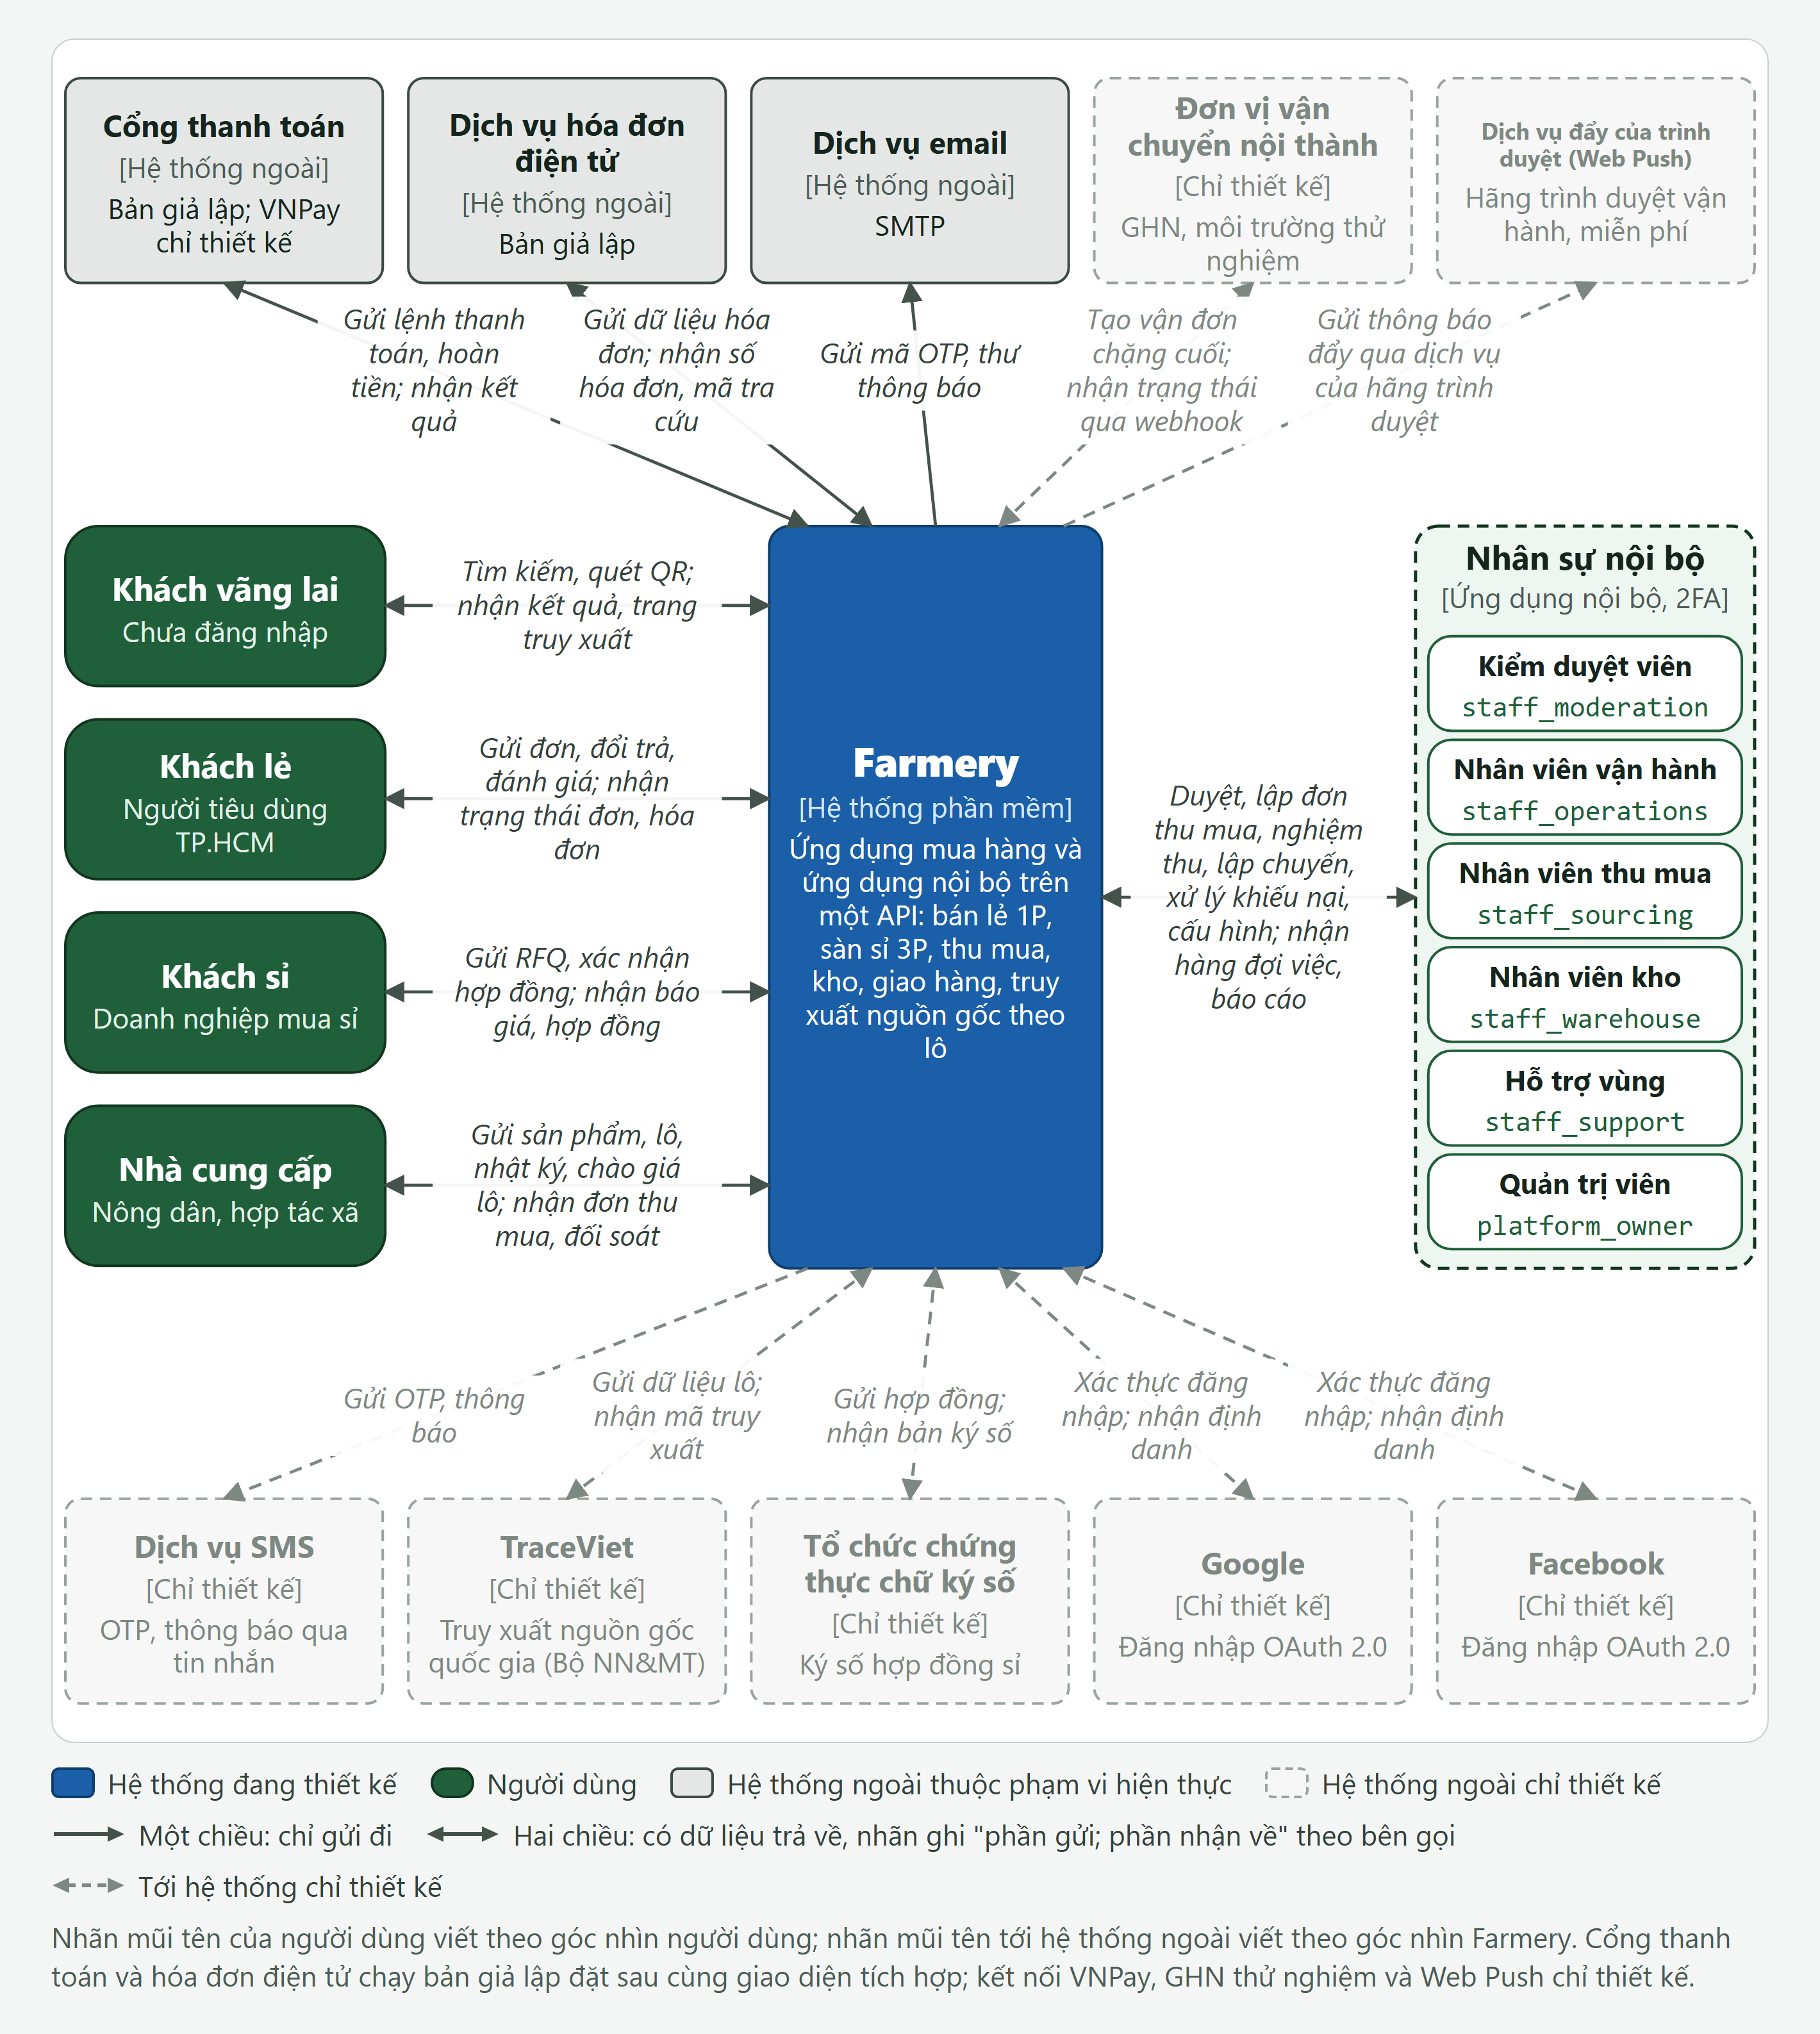
\includegraphics[width=\textwidth]{image/comparison/c4-ngu-canh.png}
\end{adjustbox}
\caption{Sơ đồ ngữ cảnh của hệ thống Farmery (C4 mức 1)}
\label{fig:c4-ngucanh}
\end{figure}

\noindent\textbf{Các nhóm người dùng.}\label{sec:doituongnguoidung} Hệ thống phục vụ ba nhóm bên ngoài và nhân sự nội bộ (Bảng~\ref{tab:nhomnguoidung}). Nhà cung cấp tham gia cả hai luồng; khách sỉ chỉ ở luồng sỉ; khách lẻ chỉ ở luồng lẻ; nhân sự nội bộ vận hành nền tảng và trực tiếp đảm nhiệm luồng bán lẻ. Tài khoản nhân sự do quản trị viên cấp; nhà cung cấp và khách sỉ qua kiểm duyệt hồ sơ (FR1.3, FR1.4); khách lẻ chỉ cần xác thực OTP.

\begingroup
\tblsetup\tblzebra
\begin{table}[H]
\centering
\small
\caption{Các nhóm người dùng và phạm vi tham gia}
\label{tab:nhomnguoidung}
\begin{tabular}{L{3.01cm} L{3.12cm} L{3.22cm} L{5.19cm}}
\toprule
\rowcolor{tblheadbg}
\textbf{Nhóm} & \textbf{Vai trò RBAC} & \textbf{Tham gia luồng} & \textbf{Khó khăn chính} \\
\midrule
Nhà cung cấp (nông dân, hợp tác xã) & \texttt{seller} & Cả hai & Hạn chế kỹ năng số và thiết bị; không đủ nhân lực xử lý từng đơn lẻ; e ngại bị ``thu phí thay thương lái'' \\
Khách sỉ (doanh nghiệp) & \texttt{buyer\_wholesale} & Bán sỉ (3P) & Khó xác minh nhiều nhà cung cấp nhỏ lẻ; rủi ro đứt cung khi mất mùa; thiếu công cụ quản lý hợp đồng \\
Khách lẻ (người tiêu dùng) & \texttt{buyer\_retail} & Bán lẻ (1P) & Khó phân biệt hàng ``sạch'' thật; lo hàng tươi hư trên đường; thói quen mua tại chợ \\
Nhân sự nội bộ & Sáu vai trò (Bảng~\ref{tab:vaitro-noibo}) & Cả hai & Quyết định lượng thu mua khi chưa chắc nhu cầu; khối lượng kiểm duyệt lớn; áp lực xử lý khiếu nại hàng dễ hỏng \\
\bottomrule
\end{tabular}
\end{table}
\endgroup

Nhân sự nội bộ chia sáu vai trò theo nguyên tắc đặc quyền tối thiểu (NFR3.1); một người có thể mang nhiều vai trò khi đội còn nhỏ. ``Quản trị viên'' chỉ chỉ vai trò \texttt{platform\_owner}. Ranh giới dễ lẫn nhất: vi phạm về \emph{nội dung} đăng bán thuộc kiểm duyệt viên, khiếu nại và tranh chấp từ một \emph{đơn hàng} thuộc nhân viên vận hành. Nhân viên hỗ trợ vùng được nhập liệu thay nhà cung cấp được phân công; mỗi lần nhập ghi người thực hiện (\texttt{entered\_by}), thời điểm, lý do và cờ \texttt{onBehalf}, nhà cung cấp xem lại được và vẫn chịu trách nhiệm tính trung thực của dữ liệu (Phụ lục~B).

\begingroup
\tblsetup\tblzebra
\begin{longtable}{L{3.30cm} L{3.60cm} L{8.00cm}}
\caption{Sáu vai trò của nhân sự nội bộ Farmery}
\label{tab:vaitro-noibo} \\
\toprule
\rowcolor{tblheadbg}
\textbf{Vai trò} & \textbf{Mã vai trò} & \textbf{Phạm vi công việc và quyền} \\
\midrule
\endfirsthead
\toprule
\rowcolor{tblheadbg}
\textbf{Vai trò} & \textbf{Mã vai trò} & \textbf{Phạm vi công việc và quyền} \\
\midrule
\endhead
\bottomrule
\endfoot
Kiểm duyệt viên & \texttt{staff\_moderation} & Duyệt hồ sơ nhà cung cấp, doanh nghiệp mua sỉ, sản phẩm, chứng nhận; duyệt đánh giá bị gắn cờ; xử lý vi phạm nội dung (FR10.1, FR10.2) \\
Nhân viên vận hành & \texttt{staff\_operations} & Xử lý khiếu nại, đổi trả, tranh chấp; giám sát đơn và giao hàng; thu hồi lô; báo cáo (FR10.3--FR10.5, FR13.6) \\
Nhân viên thu mua & \texttt{staff\_sourcing} & Xem chào giá lô, lập đơn thu mua, định giá bán lẻ, xả hàng cận hạn (FR13.1) \\
Nhân viên kho & \texttt{staff\_warehouse} & Nghiệm thu, đóng gói, in tem; quản lý dòng tồn và sổ nhập xuất; lập chuyến trung chuyển (FR13.2--FR13.4, FR8.1) \\
Nhân viên hỗ trợ vùng & \texttt{staff\_support} & Hướng dẫn và nhập liệu thay nhà cung cấp được phân công; không có quyền duyệt \\
Quản trị viên hệ thống & \texttt{platform\_owner} & Quản lý tài khoản nội bộ, vai trò; cấu hình danh mục, ngưỡng luật giám sát, biểu phí, thời hạn đổi trả, COD, giờ chốt, khung giờ giao; xem nhật ký thao tác (FR10.6, FR10.7) \\
\end{longtable}
\endgroup

\subsubsection{Chân dung khách hàng đại diện (Customer Personas)}
\label{subsec:customer-personas}

Bảng~\ref{tab:personas} trình bày bốn persona theo cách tiếp cận persona hướng mục tiêu của Cooper và cộng sự~\cite{cooper2014aboutface}; kỳ vọng ghi bằng lời người dùng, yêu cầu chỉ rút ra ở mục~\ref{sec:yeucau}. Hành trình của khách đi qua năm giai đoạn: khám phá, cân nhắc, đặt hàng, nhận hàng, đánh giá và quay lại; ở luồng lẻ khách chỉ giao dịch với Farmery, ở luồng sỉ khách giao dịch trực tiếp với từng nhà cung cấp.

\begingroup
\tblsetup\tblzebra
\begin{longtable}{L{2.60cm} L{3.90cm} L{4.20cm} L{4.20cm}}
\caption{Bốn persona đại diện}
\label{tab:personas} \\
\toprule
\rowcolor{tblheadbg}
\textbf{Persona} & \textbf{Mục tiêu} & \textbf{Điểm đau} & \textbf{Kỳ vọng ở Farmery} \\
\midrule
\endfirsthead
\toprule
\rowcolor{tblheadbg}
\textbf{Persona} & \textbf{Mục tiêu} & \textbf{Điểm đau} & \textbf{Kỳ vọng ở Farmery} \\
\midrule
\endhead
\bottomrule
\endfoot
\textbf{Bác Ba Hưng}, 52 tuổi, giám đốc HTX rau sạch Đơn Dương; Android tầm trung, 4G yếu, quen Zalo & Đầu ra ổn định, bớt phụ thuộc thương lái; hai lựa chọn tự bán sỉ hoặc bán cả lô khi cần tiền ngay & Sợ đăng bán và ghi nhật ký rườm rà; e ngại giao hàng chưa chắc nhận tiền; không có dự báo giá & Làm trọn mọi việc trên điện thoại, giao diện tối giản; QR không thêm thủ tục; có người hỗ trợ tại vùng; chắc chắn nhận tiền sau giao \\
\textbf{Chị Mai Phương}, 35 tuổi, trưởng phòng thu mua GreenMart (TP.HCM); thành thạo ERP & Nguồn cung 5--10 tấn rau củ quả đạt chuẩn mỗi tháng, giá theo sản lượng, nhận hàng nhiều đợt & Tốn thời gian thẩm định chứng nhận từng nông hộ; đứt cung do mùa vụ; chất lượng không đồng đều giữa các đợt & Hỏi giá linh hoạt, hợp đồng rõ ràng, giá giảm theo sản lượng, theo dõi từng đợt giao, báo sớm khi khan hàng \\
\textbf{Anh Minh Trí}, 29 tuổi, kỹ sư phần mềm ở Bình Thạnh, có con nhỏ; thanh toán không tiền mặt & Thực phẩm tươi, sạch, giá từ nông trại, giao nhanh trong ngày hoặc sáng hôm sau & Mất niềm tin vì rau trôi nổi gắn mác giả; lo hàng dập nát khi vận chuyển nhưng khó đổi trả & Tự kiểm tra nguồn gốc đúng lô mua; gợi ý theo mùa; đổi trả rõ ràng với một đầu mối chịu trách nhiệm \\
\textbf{Chị Thu Hà}, 27 tuổi, nhân viên thu mua Lâm Đồng; laptop ở kho, điện thoại ở ruộng & Mua đúng lượng bán được trong thời hạn bảo quản; biên lợi nhuận dương sau hao hụt & Quyết định số lượng khi chưa chắc nhu cầu; giá đổi theo ngày bào mòn biên; khó phát hiện lô tồn lâu & So sánh chào giá cùng loại; có căn cứ xu hướng giá theo mùa; tồn kho theo lô kèm hạn; báo sớm lô cận hạn \\
\end{longtable}
\endgroup

\subsection{Các vấn đề nghiên cứu}
\label{subsec:vandenghiencuu}

Bên cạnh bốn vấn đề thực tiễn ở mục~\ref{sec:vande}, Farmery đặt ra các vấn đề nghiên cứu:
\begin{enumerate}
    \item[\textbf{NC1.}] \textbf{Cơ chế uy tín chống thao túng:} tổng hợp đánh giá thành điểm phản ánh chất lượng gần đây, hạn chế dồn cụm điểm cao và đánh giá giả (mục~\ref{subsec:reputation}).
    \item[\textbf{NC2.}] \textbf{Truy xuất bất biến không dùng blockchain:} bất biến sau công khai trên cơ sở dữ liệu tập trung theo GS1, đồng bộ được với hệ thống của Nhà nước mà việc bán hàng không phụ thuộc vào đó (mục~\ref{subsec:gs1blockchain}).
    \item[\textbf{NC3.}] \textbf{Dự báo giá với dữ liệu hạn chế:} mô hình chuỗi thời gian có tính mùa vụ trên dữ liệu giá công khai.
    \item[\textbf{NC4.}] \textbf{Gợi ý khi thiếu dữ liệu tương tác (cold start):} kết hợp đặc trưng nông sản (mùa vụ, vùng trồng, chứng nhận) với hành vi người dùng.
    \item[\textbf{NC5.}] \textbf{Cân bằng hai luồng trên cùng nguồn cung:} phân bổ sản lượng giữa sỉ và lẻ, chống cam kết vượt sản lượng khi hợp đồng sỉ và đơn thu mua cùng giành một phần hàng.
\end{enumerate}
Ngưỡng chất lượng cho NC3--NC4 ở Bảng~\ref{tab:nguongAI}.

\subsection{Các thách thức và khó khăn cần được giải quyết}
\label{subsec:thachthuc}

Ba thách thức mang tính hệ thống, chi phối toàn bộ thiết kế:
\begin{itemize}
    \item \textbf{Chống bán vượt khi hai luồng dùng chung nguồn cung:} trên dòng tồn của nhà cung cấp, hợp đồng sỉ và đơn thu mua cùng giành một lượng hàng; trên dòng tồn của Farmery, nhiều đơn lẻ tranh phần còn lại. Cả hai buộc giữ chỗ và trừ tồn trong một giao dịch có khóa (NFR1.2, NFR4.1) --- ràng buộc kỹ thuật khó nhất.
    \item \textbf{Chạy được khi chưa có dữ liệu:} các mô-đun AI phải hoạt động từ ngày đầu, chưa có lịch sử tương tác hay giá nội bộ, rồi cải thiện dần.
    \item \textbf{Phụ thuộc bên không kiểm soát:} chất lượng lạnh nằm ở đối tác vận chuyển; tính xác thực chứng nhận, mã vùng trồng nằm ở cơ quan cấp chưa có giao diện tra cứu công khai; kết nối hệ thống của Bộ cần được cấp quyền; dòng tiền phải qua cổng thanh toán được cấp phép (mục~\ref{subsec:chinhsach}).
\end{itemize}

\section{Yêu cầu}
\label{sec:yeucau}

Yêu cầu xuất phát từ nhu cầu của các nhóm người dùng (mục~\ref{sec:doituongnguoidung}), được phát biểu thành user story dạng \emph{``Là ..., tôi muốn ..., để ...''} rồi truy về mã yêu cầu; danh sách đầy đủ và bảng truy vết ở Phụ lục~C. Hai ví dụ tiêu biểu: ``Là nông dân, tôi muốn bán được cả lô ngay khi thu hoạch, để không lo hàng hỏng trong lúc chờ người mua''; ``Là người tiêu dùng, tôi muốn có một nơi chịu trách nhiệm khi hàng không đạt, để không phải tự đòi từng người bán nhỏ lẻ''.

\subsection{Yêu cầu chức năng}
\label{sec:yeucauchucnang}

Các mã FRx.x đối chiếu 1--1 với use case (mục~\ref{sec:sddchitiet}) và phần hiện thực ở Chương~\ref{chap:hienthuc}. Mười ba nhóm được đánh giá theo MoSCoW, tính khả thi và phương pháp kiểm thử (Phụ lục~E): 11 nhóm ở mức Must vì thiếu nhóm nào thì trục bán lẻ đầu--cuối không chạy trọn; hai nhóm Should là tương tác người dùng (chỉ thiết kế) và hỗ trợ AI, vì khi dịch vụ AI ngưng hệ thống vẫn bán được nhờ tìm kiếm từ khóa. Dự báo giá là hạng mục duy nhất ở mức Challenging do thiếu dữ liệu giai đoạn đầu (mục~\ref{subsec:vandenghiencuu}). Bảng~\ref{tab:fr} liệt kê toàn bộ yêu cầu chức năng.

\begingroup
\tblsetup\tblzebra
\begin{longtable}{L{1.40cm} L{13.50cm}}
\caption{Danh sách yêu cầu chức năng}
\label{tab:fr} \\
\toprule
\rowcolor{tblheadbg}
\textbf{Mã} & \textbf{Yêu cầu} \\
\midrule
\endfirsthead
\toprule
\rowcolor{tblheadbg}
\textbf{Mã} & \textbf{Yêu cầu} \\
\midrule
\endhead
\bottomrule
\endfoot
\multicolumn{2}{l}{\cellcolor{tblaltbg}\textbf{FR1. Tài khoản và phân quyền}} \\
FR1.1 & Đăng ký, đăng nhập theo vai trò riêng, bằng email; đăng nhập bằng số điện thoại hoặc mạng xã hội (OAuth 2.0) \emph{(chỉ thiết kế)}. \\
FR1.2 & Xác thực OTP khi đăng ký, khôi phục mật khẩu và thao tác nhạy cảm. \\
FR1.3 & Đăng ký doanh nghiệp mua sỉ kèm giấy phép kinh doanh và mã số thuế; kiểm duyệt viên xác minh trước khi cấp quyền xem bảng giá sỉ và gửi RFQ. \\
FR1.4 & Xác minh danh tính nhà cung cấp (eKYC) trước khi cấp quyền đăng bán: kiểm duyệt viên đối chiếu thủ công ảnh giấy tờ và chân dung; đối chiếu khuôn mặt tự động \emph{(chỉ thiết kế)}. \\
FR1.5 & Quản lý sổ địa chỉ giao nhận (nhiều địa chỉ, nhãn, mặc định). \\
FR1.6 & Ghi nhận đồng ý với điều khoản và chính sách bảo mật (phiên bản, thời điểm); cho xem, tải, sửa, yêu cầu xóa dữ liệu cá nhân theo thời hạn lưu bắt buộc (NFR8.2, NFR8.5). \\
\multicolumn{2}{l}{\cellcolor{tblaltbg}\textbf{FR2. Hồ sơ nhà cung cấp}} \\
FR2.1 & Thiết lập hồ sơ (tên, ảnh, mô tả, vùng trồng); hồ sơ là trang nguồn gốc công khai, không phải gian hàng riêng. \\
FR2.2 & Báo cáo doanh thu, số đơn, sản phẩm bán chạy cho nhà cung cấp \emph{(chỉ thiết kế)}. \\
FR2.3 & Nhà cung cấp theo dõi tồn kho của mình theo lô (chi tiết ở FR13). \\
FR2.4 & Khai báo loại người bán cho nghĩa vụ thuế (tự sản xuất; hộ hoặc cá nhân kinh doanh; doanh nghiệp hoặc hợp tác xã) và nhóm thuế sản phẩm, kiểm duyệt viên xác nhận; dùng cho hóa đơn (FR7.2) và khấu trừ thuế (FR7.4). \\
\multicolumn{2}{l}{\cellcolor{tblaltbg}\textbf{FR3. Chứng nhận chất lượng}} \\
FR3.1 & Tải lên chứng nhận VietGAP, GlobalGAP, hữu cơ, OCOP, HACCP kèm tệp, mã số, cơ quan cấp, ngày hết hạn. \\
FR3.2 & Kiểm duyệt viên duyệt hoặc từ chối chứng nhận trước khi hiển thị công khai. \\
FR3.3 & Theo dõi hiệu lực, tự đánh dấu hết hạn; nhắc gia hạn \emph{(chỉ thiết kế)}. \\
\multicolumn{2}{l}{\cellcolor{tblaltbg}\textbf{FR4. Sản phẩm và truy xuất nguồn gốc}} \\
FR4.1 & Đăng bán sản phẩm kèm ảnh, mô tả, đơn vị tính, giá lẻ và bảng giá sỉ theo bậc. \\
FR4.2 & Ghi nhật ký canh tác theo lô; lô được duyệt có mã QR duy nhất, ai quét cũng xem trang truy xuất không cần đăng nhập; nhân viên hỗ trợ vùng nhập thay được, ghi \texttt{entered\_by}, thời điểm, lý do, \texttt{onBehalf}. \\
FR4.3 & Giữ chỗ và trừ tồn trên đúng dòng tồn, tránh bán vượt. \\
FR4.4 & Phân loại theo danh mục đa cấp chuyên ngành nông sản. \\
FR4.5 & Tìm kiếm và lọc (giá, vùng, chứng nhận, đánh giá, còn hàng), chấp nhận gõ không dấu, sai chính tả, kết hợp tìm kiếm ngữ nghĩa (FR12.3). \\
FR4.6 & Ràng buộc hợp lệ khi đăng bán: danh mục lá thuộc cây danh mục đóng, đơn vị tính và trường bắt buộc theo danh mục, đối chiếu danh sách loại trừ. \\
FR4.7 & Tiếp nhận báo cáo của người mua về sản phẩm sai danh mục, đưa vào hàng đợi kiểm duyệt \emph{(chỉ thiết kế)}. \\
\multicolumn{2}{l}{\cellcolor{tblaltbg}\textbf{FR5. Bán lẻ (B2C)}} \\
FR5.1 & Giỏ hàng gồm sản phẩm của gian hàng bán lẻ Farmery --- bên bán duy nhất ở luồng này. \\
FR5.2 & Đặt hàng: chọn địa chỉ, khung giờ, thanh toán; hiển thị đủ tiền hàng, thuế, cước; giữ chỗ cho đơn chờ thanh toán và tự nhả khi quá hạn; đơn sau giờ chốt vào chuyến kế tiếp. \\
FR5.3 & Mã giảm giá của gian hàng bán lẻ \emph{(chỉ thiết kế)}. \\
FR5.4 & Theo dõi đơn trên dòng thời gian tám trạng thái; hủy đơn trước đóng gói; Farmery chịu trách nhiệm trực tiếp với khách lẻ. \\
FR5.5 & Đánh giá sản phẩm sau khi đơn hoàn tất, điểm tổng hợp vào uy tín nhà cung cấp gốc; Farmery phản hồi công khai một lần dưới mỗi đánh giá \emph{(chỉ thiết kế)}. \\
FR5.6 & Mua lại: tạo giỏ mới từ sản phẩm của đơn cũ, chỉ lấy sản phẩm còn bán. \\
FR5.7 & Đăng ký nhận thông báo khi sản phẩm có hàng hoặc vào mùa \emph{(chỉ thiết kế)}. \\
\multicolumn{2}{l}{\cellcolor{tblaltbg}\textbf{FR6. Bán sỉ (B2B)}} \\
FR6.1 & Doanh nghiệp mua sỉ gửi RFQ cho một hoặc nhiều nhà cung cấp, nêu số lượng, thời gian giao, tiêu chuẩn chất lượng. \\
FR6.2 & Nhà cung cấp phản hồi một báo giá (giá bậc, số lượng, ngày giao); bên mua chấp nhận hoặc từ chối; thương lượng nhiều vòng \emph{(chỉ thiết kế)}. \\
FR6.3 & Khi báo giá được chấp nhận, hệ thống sinh hợp đồng một lần từ mẫu chuẩn; hai bên xác nhận giao kết bằng mã dùng một lần qua email, hệ thống lưu tài khoản, thời điểm, mã băm văn bản; giao một đợt, thanh toán qua cổng khi bên mua xác nhận nhận hàng; nhiều phiên bản hợp đồng \emph{(chỉ thiết kế)}. \\
FR6.4 & Tự áp khung giá sỉ khi đạt MOQ thỏa thuận trong hợp đồng. \\
FR6.5 & Lịch giao nhiều đợt trên một hợp đồng \emph{(chỉ thiết kế)}. \\
\multicolumn{2}{l}{\cellcolor{tblaltbg}\textbf{FR7. Thanh toán, hóa đơn và thuế}} \\
FR7.1 & Chuyển khoản, VietQR, ví điện tử qua cổng trung gian được cấp phép, và COD có điều kiện; hoàn tiền qua cổng theo quyết định khiếu nại. Bản hiện thực dùng cổng giả lập; kết nối VNPay thử nghiệm và IPN \emph{(chỉ thiết kế)}. \\
FR7.2 & Phát hành hóa đơn điện tử cho đơn lẻ khi hoàn tất, kèm mã tra cứu (bản giả lập); kết nối nhà cung cấp thật \emph{(chỉ thiết kế)}. \\
FR7.3 & Ký quỹ cho đơn sỉ vượt ngưỡng: tiền giữ tại cổng trung gian, giải ngân sau khi bên mua xác nhận nhận đủ hàng \emph{(chỉ thiết kế)}. \\
FR7.4 & Đối soát đơn sỉ: tính hoa hồng, xuất hóa đơn dịch vụ; khấu trừ và nộp thuế thay nhà cung cấp là hộ, cá nhân kinh doanh \emph{(chỉ thiết kế)}. \\
\multicolumn{2}{l}{\cellcolor{tblaltbg}\textbf{FR8. Giao hàng và khiếu nại}} \\
FR8.1 & Giao đơn lẻ ba chặng: nhà cung cấp tự đưa hàng về kho; nhân viên kho lập chuyến trung chuyển xe lạnh sau giờ chốt và cập nhật trạng thái; chặng cuối giao theo khung giờ khách chọn, nhân viên vận hành chuyển trạng thái; vận đơn và webhook 3PL \emph{(chỉ thiết kế)}. \\
FR8.2 & Tính phí giao gồm cước 3PL và phần bù chặng giữa, miễn khi vượt ngưỡng, hiển thị trước khi xác nhận đơn. \\
FR8.3 & Đổi trả, hoàn tiền, khiếu nại theo chính sách: thời hạn theo nhóm hàng, minh chứng ảnh hoặc video, hoàn tiền không cần trả hàng dưới ngưỡng (ghi bút toán hủy); quyết định trong thời hạn cam kết (FR10.3). \\
\multicolumn{2}{l}{\cellcolor{tblaltbg}\textbf{FR9. Tương tác người dùng}} \\
FR9.1 & Trao đổi bất đồng bộ gắn với đơn hoặc khiếu nại giữa khách và nhân viên vận hành \emph{(chỉ thiết kế)}; không có nhắn tin tự do giữa người dùng. \\
FR9.2 & Danh sách sản phẩm yêu thích \emph{(chỉ thiết kế)}. \\
\multicolumn{2}{l}{\cellcolor{tblaltbg}\textbf{FR10. Vận hành và quản trị}} \\
FR10.1 & Duyệt hồ sơ nhà cung cấp và doanh nghiệp mua sỉ, kiểm duyệt định kỳ sản phẩm, chứng nhận; khóa, mở tài khoản vi phạm. \\
FR10.2 & Giám sát vi phạm (sản phẩm sai thông tin, đánh giá giả, gian lận đơn). \\
FR10.3 & Hàng đợi khiếu nại, đổi trả có hạn xử lý, tự nâng ưu tiên khi quá hạn; phân xử khi có tranh chấp. \\
FR10.4 & Báo cáo thống kê tổng quan (giá trị giao dịch, người dùng hoạt động, tỷ lệ hoàn tất) \emph{(chỉ thiết kế)}. \\
FR10.5 & Bảng giám sát tồn kho và giao hàng: lô sắp hết hạn hoặc tồn thấp, chuyến trong ngày, đơn trễ và sự cố. \\
FR10.6 & Cấu hình: cây danh mục, ngưỡng luật giám sát, biểu phí, thời hạn khiếu nại, ngưỡng hoàn tiền không cần trả hàng, COD, giờ chốt, khung giờ giao, ngưỡng miễn cước; tạo tài khoản nội bộ và gán vai trò. \\
FR10.7 & Ghi nhật ký thao tác nhân sự có tác động tới dữ liệu người dùng (duyệt, khóa, phân xử, thu hồi, nhập thay) kèm người thực hiện, thời điểm, lý do; nhà cung cấp xem được thao tác làm thay mình. \\
\multicolumn{2}{l}{\cellcolor{tblaltbg}\textbf{FR11. Thông báo}} \\
FR11.1 & Thông báo web và email mỗi lần đơn, đổi trả, khiếu nại, RFQ, hợp đồng đổi trạng thái; thông báo đẩy, báo hàng về (FR5.7) và SMS \emph{(chỉ thiết kế)}. \\
FR11.2 & Cảnh báo chứng nhận sắp hết hạn và tồn chạm ngưỡng tối thiểu \emph{(chỉ thiết kế)}. \\
\multicolumn{2}{l}{\cellcolor{tblaltbg}\textbf{FR12. Hỗ trợ AI} (thiết kế ở mục~\ref{sec:thietkeAI})}\label{subsec:FR-AI} \\
FR12.1 & Gợi ý sản phẩm tương tự ở trang chi tiết theo độ gần vector mô tả; cá nhân hóa theo lịch sử là bước sau khi đủ dữ liệu. \\
FR12.2 & Dự báo xu hướng giá theo mùa vụ, chạy offline và đo MAPE; hiển thị cho nhân viên thu mua \emph{(chỉ thiết kế)}. \\
FR12.3 & Tìm kiếm theo ngữ nghĩa hiểu câu tự nhiên (``rau ăn lẩu'', ``trái cây ít ngọt''); tìm nhà cung cấp theo ngữ nghĩa cho khách sỉ \emph{(chỉ thiết kế)}. \\
\multicolumn{2}{l}{\cellcolor{tblaltbg}\textbf{FR13. Thu mua và quản lý kho (luồng 1P)}} \\
FR13.1 & Nhân viên thu mua lập đơn thu mua từ chào giá lô; đơn có hiệu lực khi nhà cung cấp xác nhận, từ đó sản lượng được giữ chỗ. \\
FR13.2 & Nhân viên kho nghiệm thu, ghi phần đạt, phần từ chối, hao hụt; phần đạt thành dòng tồn của Farmery, giữ mã lô, nhật ký, QR. \\
FR13.3 & Quản lý tồn theo dòng tồn (lô, chủ sở hữu, nơi chứa); mọi thay đổi qua sổ nhập xuất theo nguồn giao dịch, không sửa trực tiếp số tồn. \\
FR13.4 & Đóng gói thành đơn vị bán lẻ trong một bước, in tem QR và nhãn bắt buộc, ghi hao hụt; sơ chế nhiều bước và kiểm kê \emph{(chỉ thiết kế)}. \\
FR13.6 & Thu hồi lô: khóa mọi dòng tồn của lô ở cả hai luồng, lập danh sách đơn đã bán, thông báo người mua, hiện cảnh báo trên trang truy xuất. \\
\end{longtable}
\endgroup

\subsection{Yêu cầu phi chức năng}
\label{sec:yeucauphichucnang}

Mỗi ngưỡng truy được về một nhu cầu cụ thể của người dùng chứ không lấy từ thông lệ kỹ thuật: ngưỡng thời gian phản hồi xuất phát từ việc nhà cung cấp thao tác trên 4G không ổn định, ngưỡng khả dụng xuất phát từ điểm đau ``ngại biểu mẫu phức tạp''. Bảng~\ref{tab:nfr} liệt kê toàn bộ yêu cầu phi chức năng; chỉ số và căn cứ của từng ngưỡng ở Bảng~\ref{tab:nguongNFR} (Phụ lục~E).\label{subsec:nguongNFR} Bảy nhóm (NFR1, 3, 4, 5, 7, 8, 9) ở mức Must --- khó nhất là chống bán vượt (NFR1.2) và chịu tải 100 người dùng đồng thời (NFR1.1); NFR2, NFR6 ở mức Should; NFR2.2 chỉ thiết kế nên mức Could. Yêu cầu định tính, tuân thủ pháp lý (NFR3.4, NFR5.1, NFR8.1--8.5) và yêu cầu chỉ thiết kế được nghiệm thu bằng checklist hoặc rà soát thiết kế thay vì chỉ số đo.

\begingroup
\tblsetup\tblzebra
\begin{longtable}{L{1.40cm} L{13.50cm}}
\caption{Danh sách yêu cầu phi chức năng}
\label{tab:nfr} \\
\toprule
\rowcolor{tblheadbg}
\textbf{Mã} & \textbf{Yêu cầu} \\
\midrule
\endfirsthead
\toprule
\rowcolor{tblheadbg}
\textbf{Mã} & \textbf{Yêu cầu} \\
\midrule
\endhead
\bottomrule
\endfoot
NFR1.1 & Hiệu năng: tải trang chủ, tìm kiếm, lọc ở mức chấp nhận được kể cả với 100 người dùng đồng thời; ảnh phục vụ dạng WebP nhiều kích cỡ (đo ở mục~\ref{sec:danhgiahieunang}). \\
NFR1.2 & Không bán vượt tồn khi nhiều giao dịch đồng thời trên một dòng tồn (đơn lẻ, hợp đồng sỉ cùng đơn thu mua). \\
NFR2.1 & Mở rộng: bổ sung vai trò, mô-đun, kênh bán mới mà không đổi lớn hệ thống; vai trò là tập quyền độc lập, tài khoản mang nhiều vai trò. \\
NFR2.2 & Thành phần tải cao (tìm kiếm, đặt hàng) có thể mở rộng theo chiều ngang \emph{(chỉ thiết kế)}. \\
NFR3.1 & Phân quyền RBAC theo nguyên tắc đặc quyền tối thiểu. \\
NFR3.2 & Mã hóa dữ liệu nhạy cảm khi lưu (định danh, MST, ảnh giấy tờ eKYC, hợp đồng); tệp riêng tư chỉ đọc qua đường dẫn có chữ ký, hết hạn ngắn. \\
NFR3.3 & Băm mật khẩu bằng Bcrypt hoặc Argon2. \\
NFR3.4 & Thanh toán ủy quyền cho cổng trung gian đạt chuẩn PCI-DSS; hệ thống không lưu dữ liệu thẻ. \\
NFR3.5 & Giới hạn tần suất với hành vi có nguy cơ gian lận (đặt đơn ảo, đăng nhập sai nhiều lần). \\
NFR3.6 & Ứng dụng nội bộ bắt buộc xác thực hai lớp, phiên ngắn, có thể giới hạn theo địa chỉ mạng; API nội bộ tách tiền tố và có lớp kiểm tra quyền riêng. \\
NFR4.1 & Thao tác ảnh hưởng tồn và số dư (đặt, hủy, hoàn tiền) nhất quán trong một giao dịch cơ sở dữ liệu. \\
NFR4.2 & Sao lưu định kỳ dữ liệu hệ thống. \\
NFR5.1 & Mã nguồn tổ chức theo mô-đun tách biệt theo nghiệp vụ. \\
NFR5.2 & Tài liệu hóa API theo OpenAPI cho các endpoint chính. \\
NFR6.1 & Giao diện đơn giản, hướng dẫn rõ cho nông dân và hợp tác xã, ưu tiên hiển thị tốt trên di động (TCR $\ge 80\%$, Phụ lục~E). \\
NFR6.2 & Nhân viên hỗ trợ vùng hướng dẫn và nhập liệu thay khi cần. \\
NFR6.3 & Luồng đăng bán và ghi nhật ký tối giản, giảm số bước nhập liệu. \\
NFR7.1 & Tích hợp RESTful với vận chuyển và thanh toán qua lớp tích hợp có thời gian chờ và thử lại; bản hiện thực kiểm với cổng giả lập, kết nối thật \emph{(chỉ thiết kế)}. \\
NFR7.2 & Giao diện đáp ứng, chạy tốt trên các trình duyệt phổ biến. \\
NFR7.3 & Ứng dụng mua hàng là PWA: cài được, ghi nhật ký offline rồi đồng bộ; ứng dụng nội bộ dùng được trên điện thoại cho nhân viên kho và hỗ trợ vùng. \\
NFR8.1 & Tuân thủ Luật Thương mại điện tử 2025 với cả hai vai trò: công khai chủ quản và chính sách, người dùng đồng ý trước khi mở tài khoản, xác thực người bán, kiểm duyệt trước hiển thị, công khai nhãn bắt buộc. \\
NFR8.2 & Tuân thủ Luật Bảo vệ dữ liệu cá nhân 2025: thu thập có đồng ý, đúng mục đích, tối thiểu; chủ thể xem, sửa, xóa được (FR1.6). \\
NFR8.3 & Hóa đơn điện tử đúng nội dung và thời điểm; bản hiện thực dùng hóa đơn giả lập. \\
NFR8.4 & Khấu trừ, nộp thuế thay nhà cung cấp là hộ, cá nhân kinh doanh trên sàn sỉ \emph{(chỉ thiết kế)}. \\
NFR8.5 & Lưu dữ liệu hợp đồng ít nhất 3 năm, nhãn, chứng từ, hóa đơn ít nhất 5 năm; trong thời hạn này yêu cầu xóa dữ liệu cá nhân chỉ thực hiện bằng ẩn danh phần không bắt buộc lưu. \\
NFR9.1 & Nhật ký canh tác và chứng nhận đã duyệt, công khai thì bất biến: chỉnh sửa phải kiểm soát chặt, đính chính tạo bản ghi mới (mục~\ref{subsec:gs1blockchain}). \\
\end{longtable}
\endgroup

\subsection{Yêu cầu dữ liệu}
\label{subsec:yeucaudulieu}

Dữ liệu chia các miền sau, làm cơ sở thiết kế cơ sở dữ liệu ở mục~\ref{sec:csdl}:
\begin{itemize}
    \item \textbf{Định danh và phân quyền:} tài khoản, mã băm mật khẩu, vai trò RBAC, hồ sơ doanh nghiệp và eKYC. \textbf{Danh mục và sản phẩm:} cây danh mục đóng, đơn vị tính, giá lẻ, giá sỉ theo bậc, vùng trồng, mùa vụ.
    \item \textbf{Truy xuất và chứng nhận:} định danh lô, nhật ký canh tác theo mốc thời gian, hồ sơ chứng nhận kèm hiệu lực, mã QR theo nguyên lý GS1.
    \item \textbf{Thu mua, giao dịch, vận chuyển, tồn kho:} chào giá, đơn thu mua, nghiệm thu, giá vốn và hao hụt theo lô; đơn lẻ, RFQ, hợp đồng kèm mã băm, thanh toán, hoàn tiền, hóa đơn; chuyến trung chuyển, lịch sử trạng thái, tồn theo lô kèm hạn dùng.
    \item \textbf{Uy tín, tệp, tuân thủ, quản trị:} đánh giá và điểm uy tín; tệp công khai hoặc riêng tư kèm mã băm, thời hạn lưu; lần đồng ý chính sách, loại người bán, nhóm thuế; nhật ký thao tác và hồ sơ vi phạm.
    \item \textbf{Phân tích và học máy:} nhật ký sự kiện hành vi, chuỗi giá và sản lượng theo vùng, cảnh báo của luật ngưỡng kèm phán quyết của nhân sự (tích lũy làm nhãn cho giai đoạn sau).
\end{itemize}
Các ràng buộc chính: \emph{nhất quán giao dịch} --- giữ chỗ, trừ, nhả tồn và thay đổi tiền thực thi trong một transaction, tồn khả dụng không âm; \emph{bất biến} --- nhật ký canh tác và chứng nhận đã duyệt chỉ thêm bản ghi mới kèm người sửa và lý do; \emph{truy được giá vốn} --- mỗi đơn lẻ truy về đúng lô thu mua. Về bảo mật: dữ liệu nhạy cảm mã hóa AES-256, mật khẩu băm Bcrypt (cost $\ge 10$), không lưu thẻ (NFR3.4), snapshot hằng ngày (RPO $\le 24$h, RTO $\le 4$h), dữ liệu giao dịch sau 1 năm chuyển lưu trữ lạnh nhưng vẫn truy cập được trong thời hạn lưu bắt buộc (NFR8.5). Với AI: gợi ý tương tự dựa trên vector mô tả và đặc trưng tĩnh nên chạy được khi chưa có lịch sử tương tác; chuỗi giá cần nội suy giá trị khuyết, làm mịn đột biến và gắn nhãn theo tuần, tháng. Đặc tả thực thể ở mục~\ref{sec:csdl}.
